\documentclass[11pt]{article}
\usepackage{preamble}
\usepackage{gset}
\def\week{7}
\def\theproblem{К\week.\arabic{problem}}
\begin{document}
	\setcounter{problem}{0}
	\def\theproblem{Д\week.\arabic{problem}}
	{\textbf{\large Дискретная математика}\hfill \textbf{(Основной поток)}
		
		\medskip %
		
		\textbf{Домашнее задание \week}}
	
	\medskip
	
	\textbf{Дайте обоснованные ответы на следующие вопросы.}
	
	
	\vspace{5mm}
	
	\p В группе 40 туристов. Из них 20 человек знают английский язык,
	15~"--- французский, 11~"--- испанский. Английский и французский знают
	7 человек, английский и испанский~"--- 5, французский и испанский~"---
	3. Двое туристов знают все три языка. Сколько человек в группе не
	знает ни одного из этих языков? 
	
	Проще всего будет изобразить группу с помощью диаграммы Эйлера-Венна. \sspace
	
	\[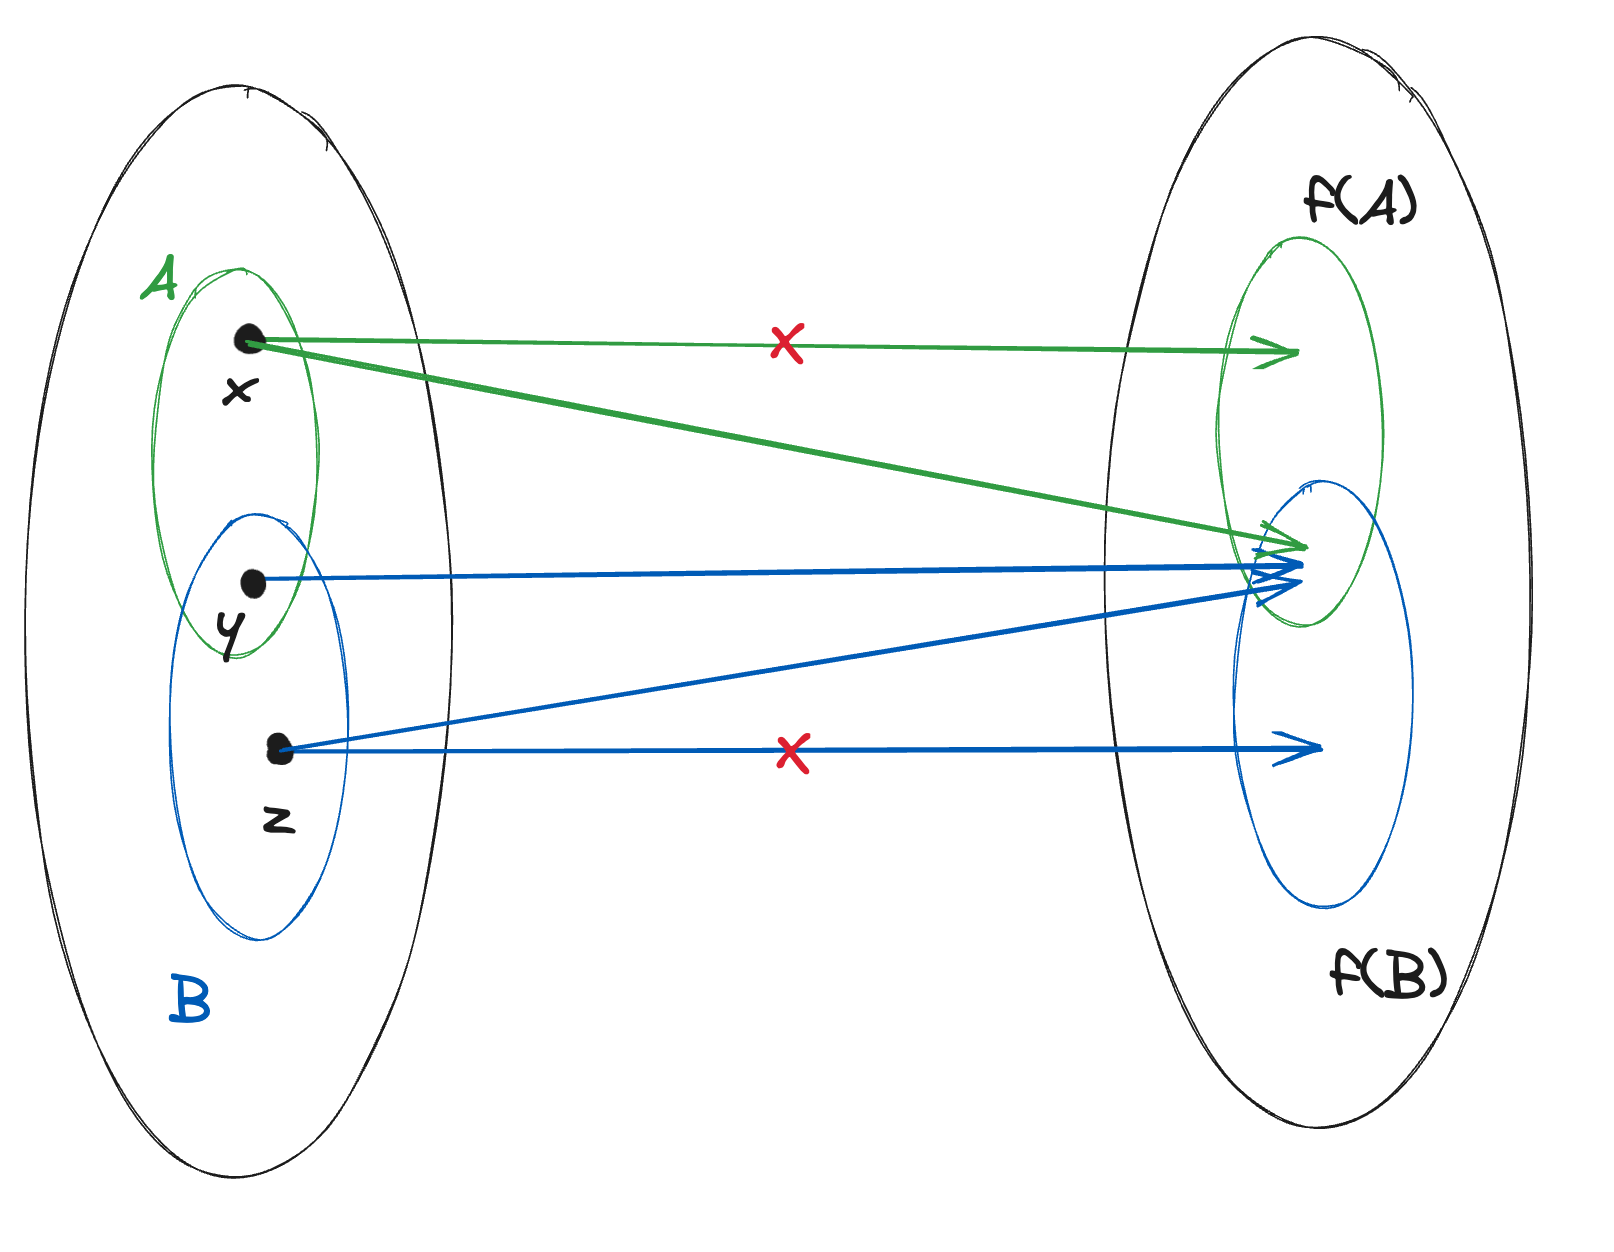
\includegraphics[width=150mm]{img1}\] \sspace
	Получается, что тех, кто не знает ни одного языка, $40 - 6 - 5 - 2 - 7 - 1 - 3 - 3 = 13$
	\sspace	
	\answer{13}
	\sspace
	
	\p Есть 3 гвоздики, 4 розы и 5 тюльпанов.
	Сколькими способами
	можно составить букет из 7 цветов, используя  имеющиеся цветы?
	(Цветы одного сорта считаем одинаковыми.)
	
	Ответом должно быть число в десятичной записи.
	
	Зная, сколько гвоздик и сколько роз можно однозначно понять, сколько нужно доложить тюльпанов, чтобы получить букет из 7 цветов. Главное, чтобы количество гвоздик + роз было $\geq 2$, потому что иначе не хватит тюльпанов, чтобы дополнить букет до 7 цветов. Всего вариантов выбрать количество гвоздик и роз $4 * 5 = 20$ способов, из них не подойдут под условие пары (0, 0) (0,1) (1,0) - 3 пары. Остается 17 вариантов. \sspace
	\answer{17}
	
	\p Сколько двоичных слов длины 12 содержат подслово 1100?
	\emph{Подслово}~"--- это последовательность стоящих подряд символов.
	Ответ должен быть целым числом в десятичной записи.
	
   Так как можно построить биекцию между словами, которые содержат 1100 в слова, которые содержат 1000, то можем рассматривать в этой задаче слова, которые содержат 1000 в качестве подслова, потому что их столько же. Биекцию можно построить, если во всех подсловах 1000 и 1100 перевернуть второй бит, при этом запомнить, где встречались подслова и дальше искать подслова только в этих местах. Иными словами, чтобы не получилось 11100 - 11000 - 10000. После первого применения функции мы запомним все биты, которые меняли и будем дальше работать только с ними, другие не будем менять ни при каких обстоятельствах. Посчитаем, сколько слов длины n не содержат 1000, назовем это функцией $f(n)$. Слова, которые меньше 4 символов всегда не содержат, поэтому $f(1) = 2, f(2) = 4, f(3) = 8$. Дальше для $n \geq 4$, если слово заканчивается на 1, то подходит $f(n - 1)$ слов, если слово заканчивается на 10, то подходит $f(n - 2)$ слов, если заканчивается на 100, то подходит $f(n - 3)$ слов, если на 000, то подходит только 1 слово из всех нулей. Таким образом $f(n) = f(n - 1) + f(n - 2) + f(n - 3) + 1$. Может посчитать, что $f(12) = 2031$. Теперь чтобы посчитать количество слов длины 12, которые содержат подстроку, надо вычесть из всех слов $f(12)$. Получим $2^{12} - 2031 = 2065$ \sspace
	\answer{2065}
	
	\p Обозначим через $S_{n,k}$ долю сюръекций из $[n]$ в $[k]$ среди всех тотальных функций из  $[n]$ в $[k]$. Докажите, что если $k = \lfloor  n/\ln n\rfloor$, то  $S_{n,k}> 0.999$ при всех достаточно больших $n$.
	
	Можно переформулировать задачу в доказательство выражения $\lim\limits_{n \to \infty} S_{n, \ln n} = 1$. \sspace
	$\lim\limits_{n \to \infty} \bigg\{S_{n, k} = \dfrac{\sum_{m = 0}^{k - 1} (-1)^m * C_m^k * (k - m)^n}{k^n} = \bs = \dfrac{\dfrac{k!}{0!(k - 0)!}* (k - 0)^n - \dfrac{k!}{1!(k  - 1)!} * (k - 1)^n + \cdots + \dfrac{1}{1!(k - 1)!} * (1)^n}{k^n} = \bs = \dfrac{1 - \dfrac{k!}{1!(k  - 1)!} * \dfrac{(k - 1)^n}{k^n} + \cdots + \dfrac{1}{1!(k - 1)!} * \dfrac{1}{k^n}}{1} = \dfrac{1 - 0 + 0 - \cdots + 0}{1}\bigg\}$ = 1 \bs
	Значит, по определению предела, найдется такое N, что для каждого n > N выполняется $S_{n,k} > 0.999$. 
	
\end{document}